\documentclass[12pt]{article}

\usepackage[utf8]{inputenc}
\usepackage[T1]{fontenc}
\usepackage{amsmath,amssymb}
\usepackage{graphicx}
\usepackage{bm}
\usepackage[hidelinks]{hyperref}
\usepackage[margin=2.5cm]{geometry}

% Shortcuts
\newcommand{\vk}{\bm{k}}
\newcommand{\ehat}{\hat{\bm{e}}}
\newcommand{\mr}{\langle r \rangle}
\newcommand{\svtwo}{\Sigma v^2}
\newcommand{\fflat}{f_{\mathrm{flat}}}

\begin{document}

\title{Directional coherence controls elastic wave transport
on discrete structures}
\author{Alexandru Toader\\
Independent researcher, Buz\u{a}u, Romania\\
\texttt{toader\_alexandru@yahoo.com}}
\date{}

\maketitle

\begin{abstract}
We identify directional coherence --- the spatial arrangement of edge
directions in the bonding network --- as the mechanism controlling elastic
wave transport on discrete structures.  On structures with few, periodically
assigned directions, the dynamical matrix varies strongly with wavevector,
producing dispersive bands and long-range propagation.  On structures with
many, incoherently assigned directions, phase-dependent anisotropic
contributions cancel statistically, bands flatten, and propagation is
suppressed.  Yet a local defect still redistributes energy over a finite,
system-size-independent distance.  This establishes a distinction between
propagation (ballistic, $v_g \neq 0$) and transport (finite spatial support
of the scattered response).  The transition between regimes is continuous,
not sharp.  Crystals with large unit cells approach the behavior of random
structures despite perfect periodicity.  A Fibonacci quasicrystal with
coherent directions retains 44--64\% of optimal crystal transport,
demonstrating that periodicity is not required.  The mechanism is validated
across 104~structures (19~crystallographic and 85~random) spanning five
coordination numbers.
\end{abstract}

\section{Introduction}

Phonon transport on periodic lattices is well understood through Bloch theory
and Boltzmann transport~\cite{ashcroft76,ziman60}.  On non-periodic discrete
structures --- amorphous solids, foams, biological networks --- periodicity is
absent and the standard framework does not apply.  Prior work has addressed
vibrational anomalies in disordered solids through jamming and rigidity
arguments~\cite{wyart05}, but what controls wave propagation and transport on
discrete structures without translational symmetry?

We show that the controlling variable is \emph{directional coherence}: the
number of distinct edge directions in the bonding network and whether they
are spatially arranged in a coherent (periodic) or incoherent (random)
pattern.  Directional coherence is not a single scalar quantity but reflects
the joint effect of directional diversity and spatial correlations in their
assignment.  As an operational proxy, we define the \emph{coherence ratio} as
$\svtwo_{\mathrm{shuffled}}/\svtwo_{\mathrm{original}}$: the fraction of
transport retained when edge directions are randomly reassigned across the
same graph (keeping the direction set fixed).  Coherent structures have
coherence ratio~$\ll 1$ (transport depends on assignment pattern); incoherent
structures have coherence ratio~$\approx 1$ (no pattern to destroy).  For
example, a BCC crystal with 6~directions assigned periodically has
$\svtwo = 0.017$; shuffling the same directions randomly drops it to
$0.00015$ --- a coherence ratio of~$0.0084$.

Our central claim, stated in falsifiable form: \emph{elastic wave transport
on discrete structures is controlled by the spatial coherence of
edge-direction assignments, which governs the $\vk$-dependence of the
dynamical matrix.}  If a structure's coherence ratio is~$\ll 1$, its
transport is assignment-dependent and suppressible by shuffling.  Structures
with few, periodically assigned directions retain dispersive bands and
long-range propagation.  Structures with many, incoherently assigned
directions --- whether structurally disordered or crystallographically complex
--- flatten their bands and suppress propagation entirely.

Yet a restricted notion of transport persists without propagation.  A local
defect on an incoherent structure redistributes energy over a finite distance
$\mr \approx 1$--$2$ lattice spacings, independent of system size.  This
establishes a distinction between \emph{propagation} ($v_g \neq 0$, energy
moves ballistically) and \emph{transport} (finite spatial support of the
defect-induced response).  We use the latter term strictly to denote the
spatial support of the Green's function response, not a transport coefficient
in the Boltzmann or diffusive sense.

This mechanism differs from Anderson localization~\cite{anderson58}, where
disorder in the potential on a regular lattice localizes eigenmodes spatially.
Here, eigenmodes remain extended ($\mathrm{IPR} \sim 1/N$); the suppression
is spectral (group velocities vanish), not spatial.  Periodicity is not
required: a Fibonacci quasicrystal~\cite{kohmoto83,shechtman84} with coherent directions
retains 44--64\% of optimal crystal transport despite non-periodic spacing.

Our results predict that crystalline materials with large unit cells suppress
elastic wave propagation in the same way as amorphous
materials~\cite{allen93,allen99}.  Complexity of the unit cell, not structural
disorder, is the relevant parameter for phonon engineering.  The mechanism is
validated across 104~structures (19~crystallographic and 85~random) spanning
five coordination numbers.

\section{Model}

We study elastic wave transport on discrete structures modeled as spring
networks~\cite{lubensky15}.  Each vertex carries 3~degrees of freedom
(displacement).  Edges connect nearest neighbors with tensorial springs
$K_e = k_L\,(\ehat \otimes \ehat)$, where $\ehat$ is the unit vector along
the edge and $k_L$ is the longitudinal spring constant ($k_T = 0$; purely
longitudinal coupling maximizes directional anisotropy).  The dynamical
matrix is
\begin{equation}\label{eq:H}
  H(\vk) = \sum_{\mathrm{edges}} (\ehat \otimes \ehat)\,
            e^{i\vk \cdot \bm{\delta}}
\end{equation}
where $\bm{\delta}$ is the displacement vector between connected vertices
under periodic boundary conditions.  We work in dimensionless units where
vertex mass, spring constant~$k_L$, and lattice spacing are set to~1.  The
box size~$L$ is measured in these units.

\paragraph{Defect.}
Scattering is induced by a Peierls defect: an SO(2) rotation of
strength~$\alpha = 0.5$ applied to edges crossing a disk of
radius~$R_{\mathrm{disk}} = 2.0$.  Ablation tests confirm that the SO(2)
gauge structure is essential ($\alpha = 0$ produces zero scattering); NNN
springs and vectorial DOF beyond one component are not needed.

\paragraph{FDTD.}
We use a Verlet integrator ($dt = 0.02$) with periodic boundary conditions
and time-windowed measurement.  A Gaussian wave packet is launched, and the
scattered field is computed as
$u_{\mathrm{sc}} = u_{\mathrm{defect}} - u_{\mathrm{ref}}$, the difference
between displacement fields with and without the Peierls defect, both evolved
from the same initial wavepacket.  The observable is
\begin{equation}\label{eq:mr}
  \mr = \frac{\sum_i d_i \,|u_{\mathrm{sc},i}|^2}
             {\sum_i |u_{\mathrm{sc},i}|^2}
\end{equation}
the energy-weighted mean distance of the scattered field from the defect
center.

\paragraph{Structures.}
We use 19~crystallographic structures from a validated catalog, random
Voronoi foams at $z = 3$--$8$, edge-swapped non-Voronoi graphs, and a
Fibonacci 3D quasicrystal~\cite{kohmoto83}.  Band structure quantities
($\svtwo$, $\fflat$) are measured along $\vk = [1,0,0]$; ranking is
preserved across 5~random $\vk$-directions and 3~vs.\ 10~$k$-values differ
by~1.6\%.

\paragraph{Validation.}
Energy oscillation in the Verlet integrator is below~$10^{-4}$.  Results are
insensitive to defect geometry ($R_{\mathrm{disk}} = 2.0$ is within 4.5\% of
the plateau at~$R = 2.5$), random seeds (means within~$2\sigma$ across
independent seed sets), and initial wave phase (CV~=~5.6\%).  The
infrastructure is validated on complex crystals (beta-Mn, $n_v = 130$;
Th$_3$P$_4$, $n_v = 188$) and verified to produce significant scattering
($E_{\mathrm{sc}}/E_{\mathrm{inc}} = 0.21$--$1.38$).  All simulation code is publicly available (see Data Availability).

\section{Flat bands from directional incoherence}

This section establishes the mechanism underlying all subsequent results.
Figure~\ref{fig:bands} illustrates the contrast: on a crystal (A15), bands
are dispersive; on a random structure at the same coordination, they are flat.

\begin{figure}[ht]
\centering
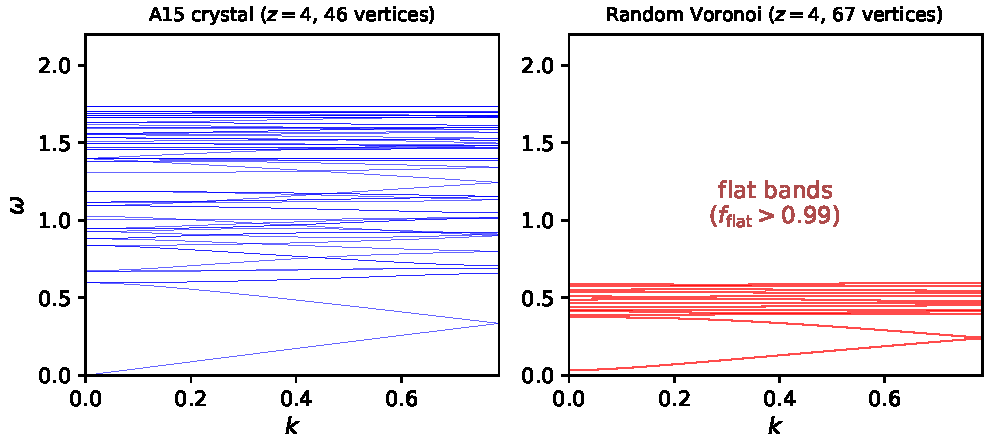
\includegraphics[width=\textwidth]{fig2_bands.pdf}
\caption{Band structure comparison. Left: A15 crystal ($z=4$, 46 vertices)
shows dispersive bands. Right: random Voronoi ($z=4$, 67 vertices) shows
flat bands ($\fflat > 0.99$). Same coordination, opposite transport.}
\label{fig:bands}
\end{figure}

Directional incoherence suppresses transport through a statistical
cancellation of phase-dependent anisotropic contributions in the dynamical
matrix~$H(\vk)$ defined in Eq.~(\ref{eq:H}).  The eigenvalues of~$H(\vk)$
determine the phonon dispersion; their variation with~$\vk$ determines group
velocities and transport.

On structures with few distinct edge directions (3--10), periodically
assigned, the sum retains strong $\vk$-dependent anisotropy: specific Bloch
phases reinforce constructively along symmetry directions, producing
dispersive bands with $\svtwo \gg 0$.  On structures with many diverse
directions~(50+), incoherently assigned, the phase-dependent anisotropic
contributions cancel statistically.  The $\vk$-dependent anisotropic
components of~$H(\vk)$ become small relative to its trace, eigenvalues become
nearly degenerate, bands flatten ($\fflat \approx 1$), and group velocities
vanish ($\svtwo \to 0$).

We verify this on 42~random structures spanning five coordination numbers
($z = 3, 4, 5, 6, 8$) and edge-swapped non-Voronoi graphs.  All give
$\fflat > 0.99$.  At the same coordination, crystals have $63\times$
(at~$z=4$) to $1097\times$ (at $z \approx 6$) larger~$\svtwo$ than random
structures.

\paragraph{Directions, not positions, control transport.}
We decouple the two contributions using a controlled test on
9~crystallographic structures.  Randomizing edge directions on a crystal graph
reduces~$\svtwo$ by $19\times$ to $338\times$.  Randomizing vertex positions
while keeping crystal directions changes~$\svtwo$ by less than a factor
of~2.  The reverse test confirms that both directions and graph topology are
necessary: crystal directions assigned to a random graph
produce~$\svtwo = 0.16\%$ of crystal.

The most direct demonstration is the \emph{shuffle test}: we take a crystal
(Kelvin/BCC), keep its exact set of 6~directions, but randomly reassign which
edge receives which direction.  The result: $\svtwo$~drops to~$0.84\%$ of
crystal --- a coherence ratio of~$0.0084$, indistinguishable from fully random
directions.  The direction set is not the variable; the spatial pattern of
assignment (periodic vs.\ random) is.

\paragraph{Gaussian decoherence.}
The decoherence follows a Gaussian law:
$\svtwo(\theta) = \svtwo_0\,\exp(-\theta^2/\sigma^2)$ where $\theta$ is the
standard deviation (in degrees) of angular noise applied to crystal edge directions.  The fit
gives $R^2 > 0.93$ on three crystals (Figure~\ref{fig:decoherence}b) (BCC $\sigma = 6.5^\circ$, diamond~$8.8^\circ$,
FCC~$8.9^\circ$).  A few degrees of directional noise collapse the band structure.
This is phenomenologically equivalent to dephasing: directional noise
progressively washes out the coherent anisotropic contributions that sustain
dispersion.

\begin{figure}[ht]
\centering
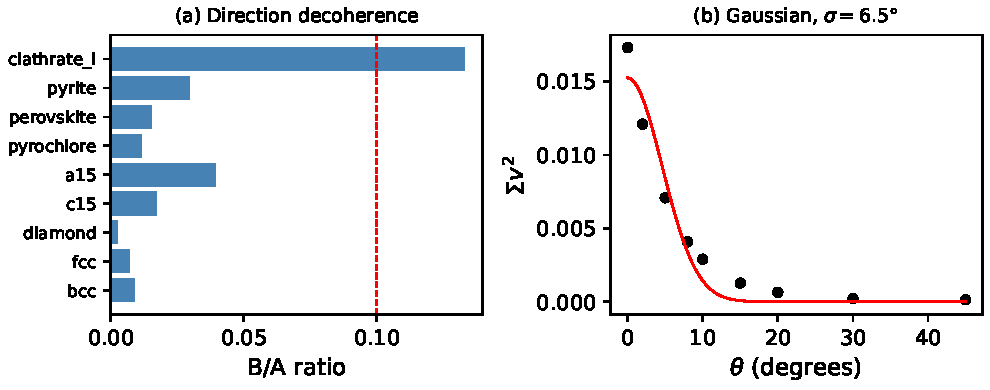
\includegraphics[width=\textwidth]{fig3_decoherence.pdf}
\caption{(a) B/A ratio ($\svtwo_{\mathrm{random\,dirs}} / \svtwo_{\mathrm{crystal\,dirs}}$)
on 9~crystals: randomizing directions reduces
$\svtwo$ by $19\times$--$338\times$. Dashed line at~0.1. clathrate\_I
(near incoherent regime) is the only structure above~0.1.
(b) Gaussian decoherence law on Kelvin: $\svtwo(\theta) \propto
\exp(-\theta^2/\sigma^2)$ with $\sigma = 6.5^\circ$.}
\label{fig:decoherence}
\end{figure}

\paragraph{Sharp suppression.}
$5\%$~edge replacement reduces~$\svtwo$ by $8.9\times$, and even
restoring~$90\%$ of crystal edges leaves~$\svtwo$ at $31\times$ below the
unperturbed crystal.  This is sharper than Anderson localization, where a
percolation-like threshold exists near~$50\%$ disorder.

\paragraph{Extended modes.}
Despite suppressed transport, eigenmodes remain spatially extended:
$\mathrm{IPR} \times n_v \approx 3$ (consistent with 3~DOF per site) at all
$k$-values tested.  This is not Anderson localization~\cite{anderson58}:
eigenmodes remain extended, and the suppression arises from spectral
flattening (group velocities vanish) rather than spatial confinement of modes.

\paragraph{Tensor average is not the variable.}
The tensor average $\langle \ehat \otimes \ehat \rangle$ does not by itself
distinguish the two regimes: Kelvin~(BCC) has
$\langle \ehat \otimes \ehat \rangle = I/3$ exactly, yet its~$\svtwo$ is
$62\times$ larger than random.  The controlling variable is not the tensor
average but the number of distinct directions and their spatial coherence ---
how they are distributed across the structure.  The flat-band result does not
depend on how directions are assigned algorithmically: on random vertex
positions, geometric directions (from $V_j - V_i$) and prescribed random
directions both give $\svtwo \ll$ crystal.

\section{Transport on coherent structures}

Having established that directional incoherence flattens bands, we now examine
the opposite limit: crystals with few coherent directions, where bands are
dispersive and $\svtwo$ predicts~$\mr$ (Figure~\ref{fig:scan}).

\begin{figure}[ht]
\centering
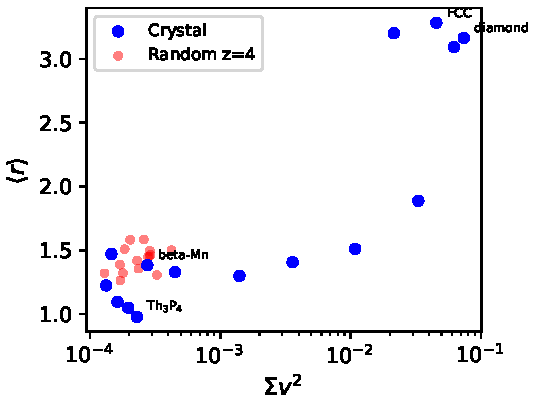
\includegraphics[width=0.7\textwidth]{fig4_scan.pdf}
\caption{$\svtwo$ vs.\ $\mr$ across 15~crystals (blue) and 15~random
$z=4$ structures (red). Crystals span from LOW transport (beta-Mn, Th$_3$P$_4$
mixed with random) to HIGH transport (FCC, diamond, $\mr > 3$). A natural
gap of~1.205 separates the two groups.}
\label{fig:scan}
\end{figure}

\paragraph{Predictive relation.}
Across 15~crystallographic structures, the Spearman correlation
between~$\svtwo$ and~$\mr$ is $\rho = 0.800$ ($p = 0.0003$).  This relation
holds across structure classes but weakens within the low-transport group (see
Limitations below).  The connection is derived from the eigenmode expansion of
the Green's function: $\mr \propto \langle v^2 \rangle / \langle v \rangle$,
verified at $\rho = 0.943$ ($p = 0.005$) on 6~crystals.

\paragraph{Classification.}
The 15~measurable crystals split into two groups separated by a natural gap
of~1.205 in~$\mr$ (between fluorite at~1.89 and perovskite at~3.09):
\begin{itemize}
  \item HIGH transport ($\mr > 3$): FCC, diamond, pyrochlore, perovskite ---
        few unique directions (4--10), $z > 5$.
  \item LOW transport ($\mr < 2$): C15, beta-Mn, gamma-brass, alpha-Mn,
        skutterudite, Th$_3$P$_4$, spinel --- many directions (34--286)
        and/or large unit cells.
\end{itemize}
Pyrite ($\mr = 1.51$ at $N=1$, $2.30$ at $N=2$; 20~dirs) and fluorite
($\mr = 1.89$; 9~dirs) are borderline.  Fluorite has few directions like HIGH
crystals but lower~$\mr$; its $\svtwo = 0.033$ overlaps with pyrochlore
($0.021$).  $\svtwo$~alone does not fully predict borderline behavior.

\paragraph{Limitations.}
Within the LOW group, the intra-group correlation
$\rho(\svtwo, \mr) = 0.455$ ($p = 0.19$) is positive but not significant at
$n = 10$.  The predictor works across groups but is weak within the LOW group.

Crystal~$\mr$ at~$N=1$ is a lower bound: $N=2$ gives $+17\%$~(A15),
$+15\%$~(C15), $+52\%$~(pyrite).  Structures with shorter edges (e.g.\
Th$_3$P$_4$, $\ell = 0.55$) have smaller absolute~$\mr$ but similar
$\mr/\ell \approx 1.8$, comparable to random ($\approx 2.0$) --- a unit
effect, not different physics.

Edge lengths are irrelevant when directions are fixed: with original crystal
directions prescribed explicitly and vertex positions perturbed,
$\svtwo$~remains identical to the unperturbed crystal (ratio~1.00).  Metric
geometry does not control transport --- only the spatial pattern of directions
matters.

SC cubic and NaCl are excluded from~$\mr$ measurements (disk geometry
incompatible with their edge structure).  Both are extreme dispersive
structures with $\svtwo = 0.66$--$2.6$.


\section{Transport without propagation}

In incoherent structures, wave propagation is suppressed ($v_g \approx 0$).
Yet a local defect still redistributes energy over a finite distance --- in
the restricted sense of~\S1.

\paragraph{System-size independence.}
We measure~$\mr$ on 100~random Voronoi foams (Figure~\ref{fig:mr_nv}) ($z=4$, 10~sizes $\times$
10~seeds, $n_v = 40$--238).  A power law fit gives $\mr \sim n_v^{-0.09}$
--- effectively constant.  This rules out a mean-free-path interpretation,
where $\mr$ would scale with domain size.  No thermodynamic limit is needed.

\begin{figure}[ht]
\centering
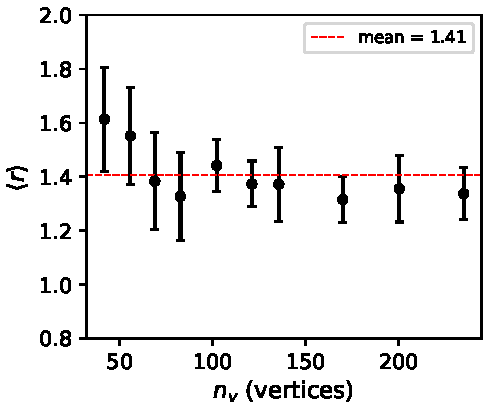
\includegraphics[width=0.7\textwidth]{fig5_mr_vs_nv.pdf}
\caption{$\mr$ vs.\ system size $n_v$ on 100~random Voronoi foams ($z=4$,
10~sizes $\times$ 10~seeds). $\mr$~is constant (mean~=~1.41, dashed line).
Error bars decrease with~$n_v$ (self-averaging).}
\label{fig:mr_nv}
\end{figure}

\paragraph{Absolute values.}
On open boundary (30~foams, $n_v$ up to~7408),
$\mr_{\mathrm{open}} = 1.52 \pm 0.05$, constant across system sizes.  On
PBC, $\mr \approx 1.4$.  FDTD measurements on random~$z=6$ ($\mr = 1.50$)
and edge-swapped non-Voronoi ($\mr = 1.74$) confirm that the result is not
$z=4$-specific; the $z=6/z=4$ ratio is~1.04.

\paragraph{Independence tests.}
$\mr$ is independent of:
\begin{itemize}
  \item Peierls strength~$\alpha$: CV~=~2.2\% across
        $\alpha = 0.05$--$0.50$.  $Z_2$~topology plays no special role on
        random structures.
  \item Band structure ($\svtwo$): at fixed~$z$, intra-$z$ Spearman
        correlations are all nonsignificant ($p > 0.05$, tested on
        5~$z$-values $\times$ 15~seeds each).  The global $\rho = 0.37$ is
        a $z$-confound artefact.
  \item Initial wave phase: CV~=~5.6\% across $k = 0.2$--$1.2$.
\end{itemize}

\paragraph{Defect size dependence.}
$\mr$ grows sublinearly with~$R_{\mathrm{disk}}$ from~1.16 ($R = 1.0$) to
1.44 ($R = 2.5$), then plateaus --- the last step gives 0\%~change.  The
observable is geometric (set by defect coupling range), not spectral.

\paragraph{Mechanism: local perturbation stays local.}
On random structures, the cosine similarity between reference and defect
fields exceeds~0.90 at $r > 3$~lattice spacings --- the fields are nearly
identical far from the defect.  On crystals at $L = 16$, the same quantity
drops to~0.45 at $r = 3$, indicating propagation.  The scattered energy
profile fits a Gaussian better than a power law, ruling out long-range tails.

$\mr$ should not be interpreted as a mean free path or diffusion length.  It
is a property of the Green's function response to a local perturbation --- the
spatial support of the scattered field --- and does not arise from asymptotic
dynamics.  This behavior is analogous to evanescent response in continuous media, but
arises here without an underlying band gap, purely from directional
incoherence.  It is distinct from the diffuson/locon classification of Allen
and Feldman~\cite{allen93,allen99} in that our modes are fully extended
($\mathrm{IPR} \sim 1/N$) yet non-propagating.


\section{The coherence continuum}

The transition from coherent to incoherent transport is continuous, not a
phase transition.

$\svtwo$ spans 4.3~orders of magnitude across our structures --- from
$\sim 0.0002$ (random) to $\sim 2.6$ (SC cubic at $N = 3$).  No binary
separator cleanly divides crystal from random: the spectral measure
$\Delta_{\mathrm{spectral}}$ shows overlap at $0.5\times$ between the lowest
crystal and highest random.  Crystals with many atoms per unit cell ---
beta-Mn (20~sites), gamma-brass~(52), alpha-Mn~(58) --- approach the
transport regime of random structures ($\mr \approx 1$--$1.5$) despite
perfect periodicity.  Beta-Mn at $\mr = 1.38$ is within $\pm 2\sigma$ of the
random distribution ($z$-score~$= -0.46$).

This is not an artefact of coordination or topology --- it is directional
diversity.  Crystal~$n_{\mathrm{dirs}}$ ranges from~4 (FCC) to~286
(alpha-Mn); random $z=4$ structures have
$n_{\mathrm{dirs}} \approx 185$--$196$.  Direction diversity varies
continuously across structures, not in discrete categories.

On controlled abstract graphs with exactly~$n_{\mathrm{dirs}}$ directions
assigned cyclically, $\svtwo$ decreases from $n_{\mathrm{dirs}} = 2$ to~3,
then saturates once $n_{\mathrm{dirs}}$ exceeds the embedding dimension.  All
values are $\ll$~crystal --- random assignment suppresses transport regardless
of how many directions are available.

Directional coherence does not reduce to a single scalar order parameter but
emerges from the interplay of directional diversity and spatial correlations
in their assignment.  The coherence ratio (defined in~\S1) is~$0.0084$ on
Kelvin, confirming that the periodic assignment pattern --- not the direction
set --- controls transport.  Partial correlation analysis confirms that
$n_{\mathrm{dirs}}$ is a proxy for~$\svtwo$, not an independent predictor
($\rho_{\mathrm{partial}} = -0.31$, $p = 0.27$).

\paragraph{Test of the theory: quasicrystals.}
A standard Fibonacci~3D quasicrystal~\cite{kohmoto83} has the same 3~edge
directions as SC cubic but non-periodic spacing ($L/S = \varphi$).  It
retains 64\% of SC transport at $n = 5$ and 44\% at $n = 6$ --- far above
random ($\sim 0.2\%$ of SC).  Periodicity is not required for transport;
directional coherence is.  Extension to other quasicrystal types
(icosahedral, Ammann-Beenker) is left for future work.


\section{Discussion}

\paragraph{Relation to Anderson localization.}
Our mechanism differs fundamentally from Anderson
localization~\cite{anderson58}.  In Anderson's picture, disorder in the
potential on a regular lattice produces spatially localized eigenmodes.  Here,
disorder is in the graph topology and edge directions, not the potential.
Eigenmodes remain spatially extended ($\mathrm{IPR} \sim 1/n_v$ at all~$k$).
The suppression is spectral --- group velocities vanish --- not spatial.

\paragraph{Complex crystals as incoherent structures.}
Any crystalline material with a sufficiently large unit cell (many atoms, many
distinct edge directions) will suppress elastic wave propagation in the same
way as an amorphous material~\cite{gelin16,baggioli19}.  This is not
disorder-driven --- it is complexity-driven.  The relevant parameter for phonon engineering is
directional diversity of the bonding network, not structural order or
periodicity.

\paragraph{Relation to hidden order and random spring networks.}
Roth and Goodwin~\cite{roth23} showed that hidden structural order in
apparently disordered crystals controls phonon band structure --- a
complementary perspective where latent order enables transport.  Our mechanism
identifies the specific structural variable (directional coherence) that
mediates this control.  On the random side, phononic band gaps in random spring
networks~\cite{spring23} have been shown to emerge from topological and
geometric disorder.  Our results show that even without band gaps, directional
incoherence alone flattens all bands and suppresses propagation.

\paragraph{Design principle.}
Our results suggest that phonon transport can be controlled by tuning
directional coherence: few, periodically arranged directions enable
propagation; many, incoherently arranged directions suppress it.  This
provides a structural design principle independent of chemical composition.

\paragraph{Connection to experiment.}
The mechanism identified here is consistent with several experimental
observations.  In amorphous silicon, Allen and Feldman~\cite{allen93,allen99}
showed that above a crossover frequency, propagating modes (propagons)
transition to diffusons --- extended modes with vanishing group velocity that
carry $\sim$93\% of the heat.  Our flat-band mechanism provides a structural
explanation for why diffusons dominate: directional incoherence of the bonding
network suppresses dispersion, producing extended but non-propagating modes.  In crystalline
materials with large unit cells, anomalously low thermal conductivity has been
reported in clathrates~\cite{takabatake14}, complex intermetallics such as
Gd$_{117}$Co$_{56}$Sn$_{112}$ ($\kappa = 0.28$~W/mK with 285~atoms per
cell)~\cite{schmitt12}, and
compounds with large unit cells where flat phonon branches appear
explicitly~\cite{cu26v2}.  In these materials, ``glass-like'' thermal
transport coexists with perfect periodicity.  Our results predict that this is
a consequence of directional diversity in the bonding network, not solely of
rattling modes or anharmonicity.

\paragraph{Scope.}
All results are for longitudinal springs ($k_T = 0$) in three dimensions.
Extension to $k_T > 0$ and 2D is expected on physical grounds (the mechanism
is spectral, not geometric) but is left for future work.

\paragraph{Limitations.}
We do not derive the Gaussian decoherence law analytically
($\svtwo(\theta) \propto \exp(-\theta^2/\sigma^2)$ is empirical with
$R^2 > 0.93$).  We do not identify a single scalar order parameter for
coherence.  The cosine similarity demonstration of local perturbation shows
weak separation on small domains ($L = 8$); clearer results require
$L \geq 16$.  Crystal~$\mr$ at $N = 1$ is a lower bound; larger supercells
would refine the classification.

\paragraph{Conclusion.}
Directional coherence, not periodicity, determines elastic wave transport on
discrete structures.

\section*{Data availability}
All data that support the findings of this study are included within
the article. Simulation code (Python) is publicly available at
\url{https://github.com/alex-toader/st_kappa}.

\begin{thebibliography}{17}
\bibitem{anderson58} P.~W.~Anderson, Phys.\ Rev.\ \textbf{109}, 1492 (1958).
\bibitem{kohmoto83} M.~Kohmoto, L.~P.~Kadanoff, C.~Tang, Phys.\ Rev.\ Lett.\ \textbf{50}, 1870 (1983).
\bibitem{ashcroft76} N.~W.~Ashcroft and N.~D.~Mermin, \emph{Solid State Physics} (Holt, 1976).
\bibitem{ziman60} J.~M.~Ziman, \emph{Electrons and Phonons} (Oxford, 1960).
\bibitem{allen93} P.~B.~Allen and J.~L.~Feldman, Phys.\ Rev.\ B \textbf{48}, 12581 (1993).
\bibitem{allen99} P.~B.~Allen, J.~L.~Feldman, J.~Fabian, F.~Wooten, Phil.\ Mag.\ B \textbf{79}, 1715 (1999).
\bibitem{wyart05} M.~Wyart, Ann.\ Phys.\ Fr.\ \textbf{30}, 1 (2005).
\bibitem{shechtman84} D.~Shechtman \emph{et al.}, Phys.\ Rev.\ Lett.\ \textbf{53}, 1951 (1984).
\bibitem{lubensky15} T.~C.~Lubensky \emph{et al.}, Rep.\ Prog.\ Phys.\ \textbf{78}, 073901 (2015).
\bibitem{gelin16} S.~Gelin, H.~Tanaka, A.~Lema\^itre, Nature Mater.\ \textbf{15}, 1177 (2016).
\bibitem{baggioli19} M.~Baggioli and A.~Zaccone, Phys.\ Rev.\ Lett.\ \textbf{122}, 145501 (2019).
\bibitem{takabatake14} T.~Takabatake, K.~Suekuni, T.~Nakayama, E.~Kaneshita, Rev.\ Mod.\ Phys.\ \textbf{86}, 669 (2014).
\bibitem{cu26v2} K.~S.~Rana \emph{et al.}, Phys.\ Rev.\ B \textbf{109}, 115202 (2024).
\bibitem{roth23} G.~A.~Roth and A.~L.~Goodwin, Nat.\ Commun.\ \textbf{14}, 4328 (2023).
\bibitem{spring23} K.~Xiong, J.~Ren, F.~Marchesoni, J.~Huang, Phys.\ Rev.\ E \textbf{108}, 044306 (2023).
\bibitem{schmitt12} D.~C.~Schmitt \emph{et al.}, J.\ Am.\ Chem.\ Soc.\ \textbf{134}, 5965 (2012).
% repo URL in Data Availability section, not duplicated here
\end{thebibliography}

\end{document}
